\documentclass[11pt, oneside]{article}   	% use "amsart" instead of "article" for AMSLaTeX format
\usepackage{geometry}                		% See geometry.pdf to learn the layout options. There are lots.
\geometry{letterpaper}                   		% ... or a4paper or a5paper or ... 
%\geometry{landscape}                		% Activate for for rotated page geometry
%\usepackage[parfill]{parskip}    		% Activate to begin paragraphs with an empty line rather than an indent
\usepackage{graphicx}				% Use pdf, png, jpg, or eps§ with pdflatex; use eps in DVI mode
								% TeX will automatically convert eps --> pdf in pdflatex		
\usepackage{amssymb}

\title{Brief Article}
\author{The Author}
%\date{}							% Activate to display a given date or no date

\begin{document}
\maketitle
%\section{}
%\subsection{}


\begin{verbatim}
import sys
sys.path.insert(0, 'lib/py/')
from inters import *
from iot3d import *
from larcc import *

filename = "test/py/inters/plan.svg"
lines = svg2lines(filename)
#VIEW(STRUCT(AA(POLYLINE)(lines)))
    
V,FV,EV = larFromLines(lines)
FV[2] += FV[71]
#VIEW(EXPLODE(1.2,1.2,1)(MKPOLS((V,FV[:-1]+EV)) + AA(MK)(V)))

VV = AA(LIST)(range(len(V)))
submodel = STRUCT(MKPOLS((V,EV)))
#VIEW(larModelNumbering(1,1,1)(V,[VV,EV,FV[:-1]],submodel,0.025))

verts,faces,edges = polyline2lar([[ V[v] for v in FV[-1] ]])
#VIEW(EXPLODE(1.2,1.2,1)(MKPOLS((verts,edges))))


verts,faces,edges


from scipy import spatial
from bool import crossRelation,pointInPolygonClassification

def subComplexInBox(V,FV,EV,queryBox):
    (xmin,ymin),(xmax,ymax) = queryBox
    if xmin > xmax: xmin,xmax = xmax,xmin
    if ymin > ymax: ymin,ymax = ymax,ymin
    vdict = dict([(vcode(vert),k) for k,vert in enumerate(V)])
    vertexSubset = [vdict[vcode((x,y))] for x,y in V if xmin<=x<=xmax and ymin<=y<=ymax]
    edgeSubset = [e for e,edge in enumerate(EV) if all([v in vertexSubset  for v in edge])]    
    faceSubset = [f for f,face in enumerate(FV) if all([v in vertexSubset  for v in face])]
    return vertexSubset,faceSubset,edgeSubset

queryPoint = (0.6,0.58)
selectBox = ((0.5, 0.5), (1, 0.75))
vertexSubset,faceSubset,edgeSubset = subComplexInBox(V,FV,EV,selectBox)
#VIEW(EXPLODE(1.2,1.2,1.2)(MKPOLS((V,[EV[e] for e in edgeSubset])) + [COLOR(RED)(MK(queryPoint))]))

   
def subComplexAroundPoint(V,FV,EV,FE,queryPoint):
    tree = spatial.cKDTree(V)
    pts = np.array([queryPoint])
    dist,closestVertex = tree.query(pts)
    VF = invertRelation(FV)
    closestFaces = VF[closestVertex]
    for face in closestFaces:
    	faceEdges = [EV[e] for e in FE[face]]
        if pointInPolygonClassification(queryPoint, (V,faceEdges)) == "p_in":
            break
    vertexSubset = FV[face]
    edgeSubset = [EV[e] for e in FE[face]]
    faceSubset = [face]
    return vertexSubset,faceSubset,edgeSubset
    
     
FE = crossRelation(FV,EV)
vertexSubset,faceSubset,edgeSubset = subComplexAroundPoint(V,FV,EV,FE,queryPoint)
#VIEW(EXPLODE(1.2,1.2,1.2)(MKPOLS((V,[EV[e] for e in FE[faceSubset[0]]])) + [COLOR(RED)(MK(queryPoint))] ))



def cells2hpcs(V,FV,cells,k): 
    return AA(COLOR(colors[k]))(MKPOLS((V,[FV[f] for f in cells])))


colors = [RED,GREEN,BLUE,CYAN,MAGENTA,YELLOW,WHITE,PURPLE,BROWN]
boxes = [0 for k in range(64)]
point = [0 for k in range(64)]
FE = crossRelation(FV,EV)

#-- ala NORD -------------------------------------------------------------------------


boxes[0] = [[0.431, 0.607], [0.474, 0.91]] #[V[k] for k in [39,208]]
boxes[1] = [[0.416, 0.657], [0.372, 0.953]] #[V[k] for k in [162,39]]
boxes[2] = [[0.416, 0.627], [0.431, 0.986]] #[V[k] for k in [206,247]]
boxes[3] = [[0.431, 0.607], [0.448, 0.627]] #[V[k] for k in [39,7]]
boxes[4] = [[0.431, 0.91], [0.494, 0.929]]  #[V[k] for k in [213,234]]
boxes[5] = [[0.431, 0.97], [0.466, 1.0]] #[V[k] for k in [58,88]]
boxes[27] = [[0.416, 0.627], [0.372, 0.657]] #[V[k] for k in [110,82]]

point[0] = [0.394, 0.9625] #CCOMB([V[k] for k in [190,197]])
point[1] = [0.4525, 0.9325] #CCOMB([V[k] for k in [166,159]])


piano1_superficieUtile_zonaNord_uffici_destra = subComplexInBox(V,FV,EV,boxes[0])[1]
piano1_superficieUtile_zonaNord_uffici_sinistra = subComplexInBox(V,FV,EV,boxes[1])[1]
piano1_connettivo_orizzontale_zonaNord = subComplexInBox(V,FV,EV,boxes[2])[1]
piano1_connettivo_verticale_zonaNord_ascensore = subComplexInBox(V,FV,EV,boxes[3])[1]
piano1_connettivo_verticale_zonaNord_ascensore += subComplexInBox(V,FV,EV,boxes[4])[1]
piano1_connettivo_verticale_zonaNord_scale = subComplexInBox(V,FV,EV,boxes[5])[1]
piano1_superficieUtile_zonaNord_servizi = subComplexAroundPoint(V,FV,EV,FE,point[0])[1]
piano1_superficieUtile_zonaNord_servizi += subComplexAroundPoint(V,FV,EV,FE,point[1])[1]
piano1_superficieUtile_zonaNord_servizi += subComplexInBox(V,FV,EV,boxes[27])[1]

piano1N = [piano1_superficieUtile_zonaNord_uffici_destra, piano1_superficieUtile_zonaNord_uffici_sinistra, piano1_connettivo_orizzontale_zonaNord, piano1_connettivo_verticale_zonaNord_ascensore, piano1_connettivo_verticale_zonaNord_scale, piano1_superficieUtile_zonaNord_servizi]
    
nord = CAT([cells2hpcs(V,FV,chain,k) for k,chain in enumerate(piano1N)])
#VIEW(EXPLODE(1.2,1.2,1.2)(nord))

#-- ala EST -------------------------------------------------------------------------

boxes[6] = [[0.019, 0.533], [0.376, 0.577]] #[V[k] for k in [241,29]]
boxes[7] = [[0.07, 0.474], [0.343, 0.518]] #[V[k] for k in [264,148]]
boxes[8] = [[0.013, 0.518], [0.376, 0.533]] #[V[k] for k in [22,63]]
boxes[9] = [[0.376, 0.533], [0.39, 0.549]] #[V[k] for k in [63,92]]
boxes[10] = [[0.001, 0.474], [0.07, 0.518]] #[V[k] for k in [263,265]]
boxes[11] = [[0.343, 0.474], [0.376, 0.518]] #[V[k] for k in [84,149]]

point[2] = [0.015, 0.5535] #CCOMB([V[k] for k in [228,14]])


piano1_superficieUtile_zonaEst_uffici_destra = subComplexInBox(V,FV,EV,boxes[6])[1]
piano1_superficieUtile_zonaEst_uffici_sinistra = subComplexInBox(V,FV,EV,boxes[7])[1]
piano1_connettivo_orizzontale_zonaEst = subComplexInBox(V,FV,EV,boxes[8])[1]
piano1_connettivo_verticale_zonaEst_ascensore = subComplexInBox(V,FV,EV,boxes[9])[1]
piano1_connettivo_verticale_zonaEst_scale = subComplexAroundPoint(V,FV,EV,FE,point[2])[1]
piano1_superficieUtile_zonaEst_servizi = subComplexInBox(V,FV,EV,boxes[10])[1]
piano1_superficieUtile_zonaEst_servizi += subComplexInBox(V,FV,EV,boxes[11])[1]

piano1E = [piano1_superficieUtile_zonaEst_uffici_destra, piano1_superficieUtile_zonaEst_uffici_sinistra, piano1_connettivo_orizzontale_zonaEst, piano1_connettivo_verticale_zonaEst_ascensore, piano1_connettivo_verticale_zonaEst_scale, piano1_superficieUtile_zonaEst_servizi]

est = CAT([cells2hpcs(V,FV,chain,k) for k,chain in enumerate(piano1E)])
#VIEW(EXPLODE(1.2,1.2,1.2)(est + nord))


#-- ala SUD -------------------------------------------------------------------------

boxes[12] = [[0.467, 0.138], [0.423, 0.476]] #[V[k] for k in [252,47]]
boxes[13] = [[0.482, 0.145], [0.525, 0.445]] #[V[k] for k in [241,126]]
boxes[14] = [[0.482, 0.476], [0.467, 0.116]] #[V[k] for k in [254,232]]
boxes[15] = [[0.449, 0.476], [0.467, 0.493]] #[V[k] for k in [40,237]]
boxes[16] = [[0.431, 0.101], [0.467, 0.131]] #[V[k] for k in [259,2]]
boxes[17] = [[0.482, 0.445], [0.525, 0.476]] #[V[k] for k in [155,248]]
boxes[18] = [[0.525, 0.104], [0.482, 0.145]] #[V[k] for k in [111,241]]

piano1_superficieUtile_zonaSud_uffici_destra = subComplexInBox(V,FV,EV,boxes[12])[1]
piano1_superficieUtile_zonaSud_uffici_sinistra = subComplexInBox(V,FV,EV,boxes[13])[1]
piano1_connettivo_orizzontale_zonaSud = subComplexInBox(V,FV,EV,boxes[14])[1]
piano1_connettivo_verticale_zonaSud_ascensore = subComplexInBox(V,FV,EV,boxes[15])[1]
piano1_connettivo_verticale_zonaSud_scale = subComplexInBox(V,FV,EV,boxes[16])[1]
piano1_superficieUtile_zonaSud_servizi = subComplexInBox(V,FV,EV,boxes[17])[1]
piano1_superficieUtile_zonaSud_servizi += subComplexInBox(V,FV,EV,boxes[18])[1]

piano1S = [piano1_superficieUtile_zonaSud_uffici_destra, piano1_superficieUtile_zonaSud_uffici_sinistra, piano1_connettivo_orizzontale_zonaSud, piano1_connettivo_verticale_zonaSud_ascensore, piano1_connettivo_verticale_zonaSud_scale, piano1_superficieUtile_zonaSud_servizi]
    
sud = CAT([cells2hpcs(V,FV,chain,k) for k,chain in enumerate(piano1S)])
#VIEW(EXPLODE(1.2,1.2,1.2)(est + nord + sud))


#-- ala OVEST -------------------------------------------------------------------------

boxes[19] = [[0.521, 0.526], [0.963, 0.568]] #[V[k] for k in [169,202]]
boxes[20] = [[0.555, 0.584], [0.955, 0.627]] #[V[k] for k in [12,23]]
boxes[21] = [[0.521, 0.568], [0.985, 0.584]] #[V[k] for k in [209,204]]
boxes[22] = [[0.506, 0.551], [0.521, 0.568]] #[V[k] for k in [89,209]]
boxes[23] = [[0.808, 0.504], [0.828, 0.526]] #[V[k] for k in [270,77]]
boxes[24] = [[0.955, 0.584], [0.997, 0.627]] #[V[k] for k in [220,24]]
boxes[25] = [[0.521, 0.584], [0.555, 0.627]] #[V[k] for k in [11,144]]
boxes[26] = [[1.0, 0.533], [0.97, 0.568]] #[V[k] for k in [233,201]]


piano1_superficieUtile_zonaOvest_uffici_destra = subComplexInBox(V,FV,EV,boxes[19])[1]
piano1_superficieUtile_zonaOvest_uffici_sinistra = subComplexInBox(V,FV,EV,boxes[20])[1]
piano1_connettivo_orizzontale_zonaOvest = subComplexInBox(V,FV,EV,boxes[21])[1]
piano1_connettivo_verticale_zonaOvest_ascensore = subComplexInBox(V,FV,EV,boxes[22])[1]
piano1_connettivo_verticale_zonaOvest_ascensore += subComplexInBox(V,FV,EV,boxes[23])[1]
piano1_superficieUtile_zonaOvest_servizi = subComplexInBox(V,FV,EV,boxes[24])[1]
piano1_superficieUtile_zonaOvest_servizi += subComplexInBox(V,FV,EV,boxes[25])[1]
piano1_connettivo_verticale_zonaOvest_scale = subComplexInBox(V,FV,EV,boxes[26])[1]

piano1O = [piano1_superficieUtile_zonaOvest_uffici_destra, piano1_superficieUtile_zonaOvest_uffici_sinistra, piano1_connettivo_orizzontale_zonaOvest, piano1_connettivo_verticale_zonaOvest_ascensore, piano1_connettivo_verticale_zonaOvest_scale, piano1_superficieUtile_zonaOvest_servizi]
    
ovest = CAT([cells2hpcs(V,FV,chain,k) for k,chain in enumerate(piano1O)])
#VIEW(EXPLODE(1.2,1.2,1.2)(est + nord + sud + ovest))


#-- CENTRO stella -------------------------------------------------------------------------

piano1_connettivo_orizzontale_centroStella = [2]
piano1_connettivo_verticale_centroStella_scale = [15,26]

piano1C = [[],[],piano1_connettivo_orizzontale_centroStella,[], piano1_connettivo_verticale_centroStella_scale]
centro = CAT([cells2hpcs(V,FV,chain,k) for k,chain in enumerate(piano1C)])
#VIEW(EXPLODE(1.2,1.2,1.2)(est + nord + sud + ovest + centro))
#VIEW(STRUCT(est + nord + sud + ovest + centro))


#-- Strutture foglia -------------------------------------------------------------------------

def chain2BoundaryChain(FV,EV):
    csrBoundaryMat = boundary(FV,EV)
    nedges,nfaces = csrBoundaryMat.shape   
    def chain2BoundaryChain0(chain):
        row = np.array(chain)
        col = np.array([0 for k in range(len(chain))])
        data = np.array([1 for k in range(len(chain))])
        csrFaceVect = scipy.sparse.coo_matrix((data, (row, col)), shape=(nfaces,1)).tocsr()
        csrEdgeVect = csrBoundaryMat*csrFaceVect
        boundaryChain = [h for h,val in 
            zip(csrEdgeVect.tocoo().row, csrEdgeVect.tocoo().data) if val%2 != 0]
        return boundaryChain
    return chain2BoundaryChain0
 
def chain2structs(V,FV,EV,FE):
    def chain2structs0(args): 
        chainName,classtype = args
        chain = eval(chainName)
        boundaryFacets = chain2BoundaryChain(FV,EV)(chain)
        ##VIEW(EXPLODE(1.2,1.2,1.2)(MKPOLS((V,[EV[e] for e in boundaryFacets]))))
        chainFacets = sorted(set(CAT([FE[cell] for cell in chain])))
        """
        if isinstance(chain,Struct): 
            V,FV,EV = struct2lar(chain)
            chain = FV
        """
        struct = []
        chainVerts = list(set(CAT([FV[cell] for cell in chain])))
        localOrigin = min([V[v] for v in chainVerts])
        for cell in chain:
            vs = (array([V[v] for v in FV[cell]]) - localOrigin).tolist()
            vdict = dict([[vcode(vert),k] for k,vert in enumerate(vs)])
            facetEdges = [ (array([V[v] for v in EV[e]]) - localOrigin).tolist() for e in FE[cell]]
            ev = [(vdict[vcode(v1)], vdict[vcode(v2)]) for v1,v2 in facetEdges]
            fv = [range(len(vs))]
            tvect = eval(min(vdict))
            shape = (array(vs)-tvect).tolist(),fv,ev
            struct += [ Struct([ t(*tvect), shape],name=None,category="room" ) ]
            out = Struct([t(*localOrigin)]+struct,name=chainName,category=classtype)
        return out
    return chain2structs0




#-- Strutture intermedie -------------------------------------------------------------------------

chainsToStruct = chain2structs(V,FV,EV,FE)

piano1N_nomi = ["piano1_superficieUtile_zonaNord_uffici_destra", "piano1_superficieUtile_zonaNord_uffici_sinistra", "piano1_connettivo_orizzontale_zonaNord", "piano1_connettivo_verticale_zonaNord_ascensore", "piano1_connettivo_verticale_zonaNord_scale", "piano1_superficieUtile_zonaNord_servizi"]
piano1N_categorie = ["uffici","uffici","corridoi","ascensori","scale","servizi"]
p1N = zip(piano1N_nomi,piano1N_categorie)
piano1_zonaNord = Struct(AA(chainsToStruct)(p1N),"piano1_zonaNord","ala")
#VIEW(SKEL_1(STRUCT(MKPOLS(struct2lar(piano1_zonaNord)))))


piano1E_nomi = ["piano1_superficieUtile_zonaEst_uffici_destra", "piano1_superficieUtile_zonaEst_uffici_sinistra", "piano1_connettivo_orizzontale_zonaEst", "piano1_connettivo_verticale_zonaEst_ascensore", "piano1_connettivo_verticale_zonaEst_scale", "piano1_superficieUtile_zonaEst_servizi"]
piano1E_categorie = ["uffici","uffici","corridoi","ascensori","scale","servizi"]
p1E = zip(piano1E_nomi, piano1E_categorie)
piano1_zonaEst = Struct(AA(chainsToStruct)(p1E), "piano1_zonaEst", "ala")
#VIEW(SKEL_1(STRUCT(MKPOLS(struct2lar(piano1_zonaEst)))))


piano1S_nomi = ["piano1_superficieUtile_zonaSud_uffici_destra", "piano1_superficieUtile_zonaSud_uffici_sinistra", "piano1_connettivo_orizzontale_zonaSud", "piano1_connettivo_verticale_zonaSud_ascensore", "piano1_connettivo_verticale_zonaSud_scale", "piano1_superficieUtile_zonaSud_servizi"]
piano1S_categorie = ["uffici","uffici","corridoi","ascensori","scale","servizi"]
p1S = zip(piano1S_nomi, piano1S_categorie)
piano1_zonaSud = Struct(AA(chainsToStruct)(p1S), "piano1_zonaSud", "ala")
#VIEW(SKEL_1(STRUCT(MKPOLS(struct2lar(piano1_zonaSud)))))


piano1O_nomi = ["piano1_superficieUtile_zonaOvest_uffici_destra", "piano1_superficieUtile_zonaOvest_uffici_sinistra", "piano1_connettivo_orizzontale_zonaOvest", "piano1_connettivo_verticale_zonaOvest_ascensore", "piano1_connettivo_verticale_zonaOvest_scale", "piano1_superficieUtile_zonaOvest_servizi"]
piano1O_categorie = ["uffici","uffici","corridoi","ascensori","scale","servizi"]
p1O = zip(piano1O_nomi, piano1O_categorie)
piano1_zonaOvest = Struct(AA(chainsToStruct)(p1O), "piano1_zonaOvest", "ala")
#VIEW(SKEL_1(STRUCT(MKPOLS(struct2lar(piano1_zonaOvest)))))


piano1C_nomi = ["piano1_connettivo_orizzontale_centroStella", "piano1_connettivo_verticale_centroStella_scale"]
piano1C_categorie = ["corridoi","ascensori"]
p1C = zip(piano1C_nomi, piano1C_categorie)
piano1_centroStella = Struct(AA(chainsToStruct)(p1C), "piano1_centroStella", "centro")
#VIEW(SKEL_1(STRUCT(MKPOLS(struct2lar(piano1_centroStella)))))


#-- Primo piano -------------------------------------------------------------------------

p1 = p1N + p1S + p1E + p1O + p1C

piano1_nomi = ["piano1_zonaNord", "piano1_zonaEst", "piano1_zonaSud", "piano1_zonaOvest", "piano1_centroStella"]
piano1_categorie = ["ala","ala","ala","ala","centro"]
piano1 = Struct(AA(chainsToStruct)(p1), "piano1", "piano")
#VIEW(SKEL_1(STRUCT(MKPOLS(struct2lar(piano1)))))




b = chain2BoundaryChain(FV,EV)()


b = chain2BoundaryChain(FV,EV)(piano1_connettivo_orizzontale_zonaNord +											piano1_connettivo_orizzontale_zonaSud + piano1_connettivo_orizzontale_zonaEst + 							piano1_connettivo_orizzontale_zonaOvest + piano1_connettivo_orizzontale_centroStella)
\end{verbatim}


\begin{figure}[htbp] %  figure placement: here, top, bottom, or page
   \centering
   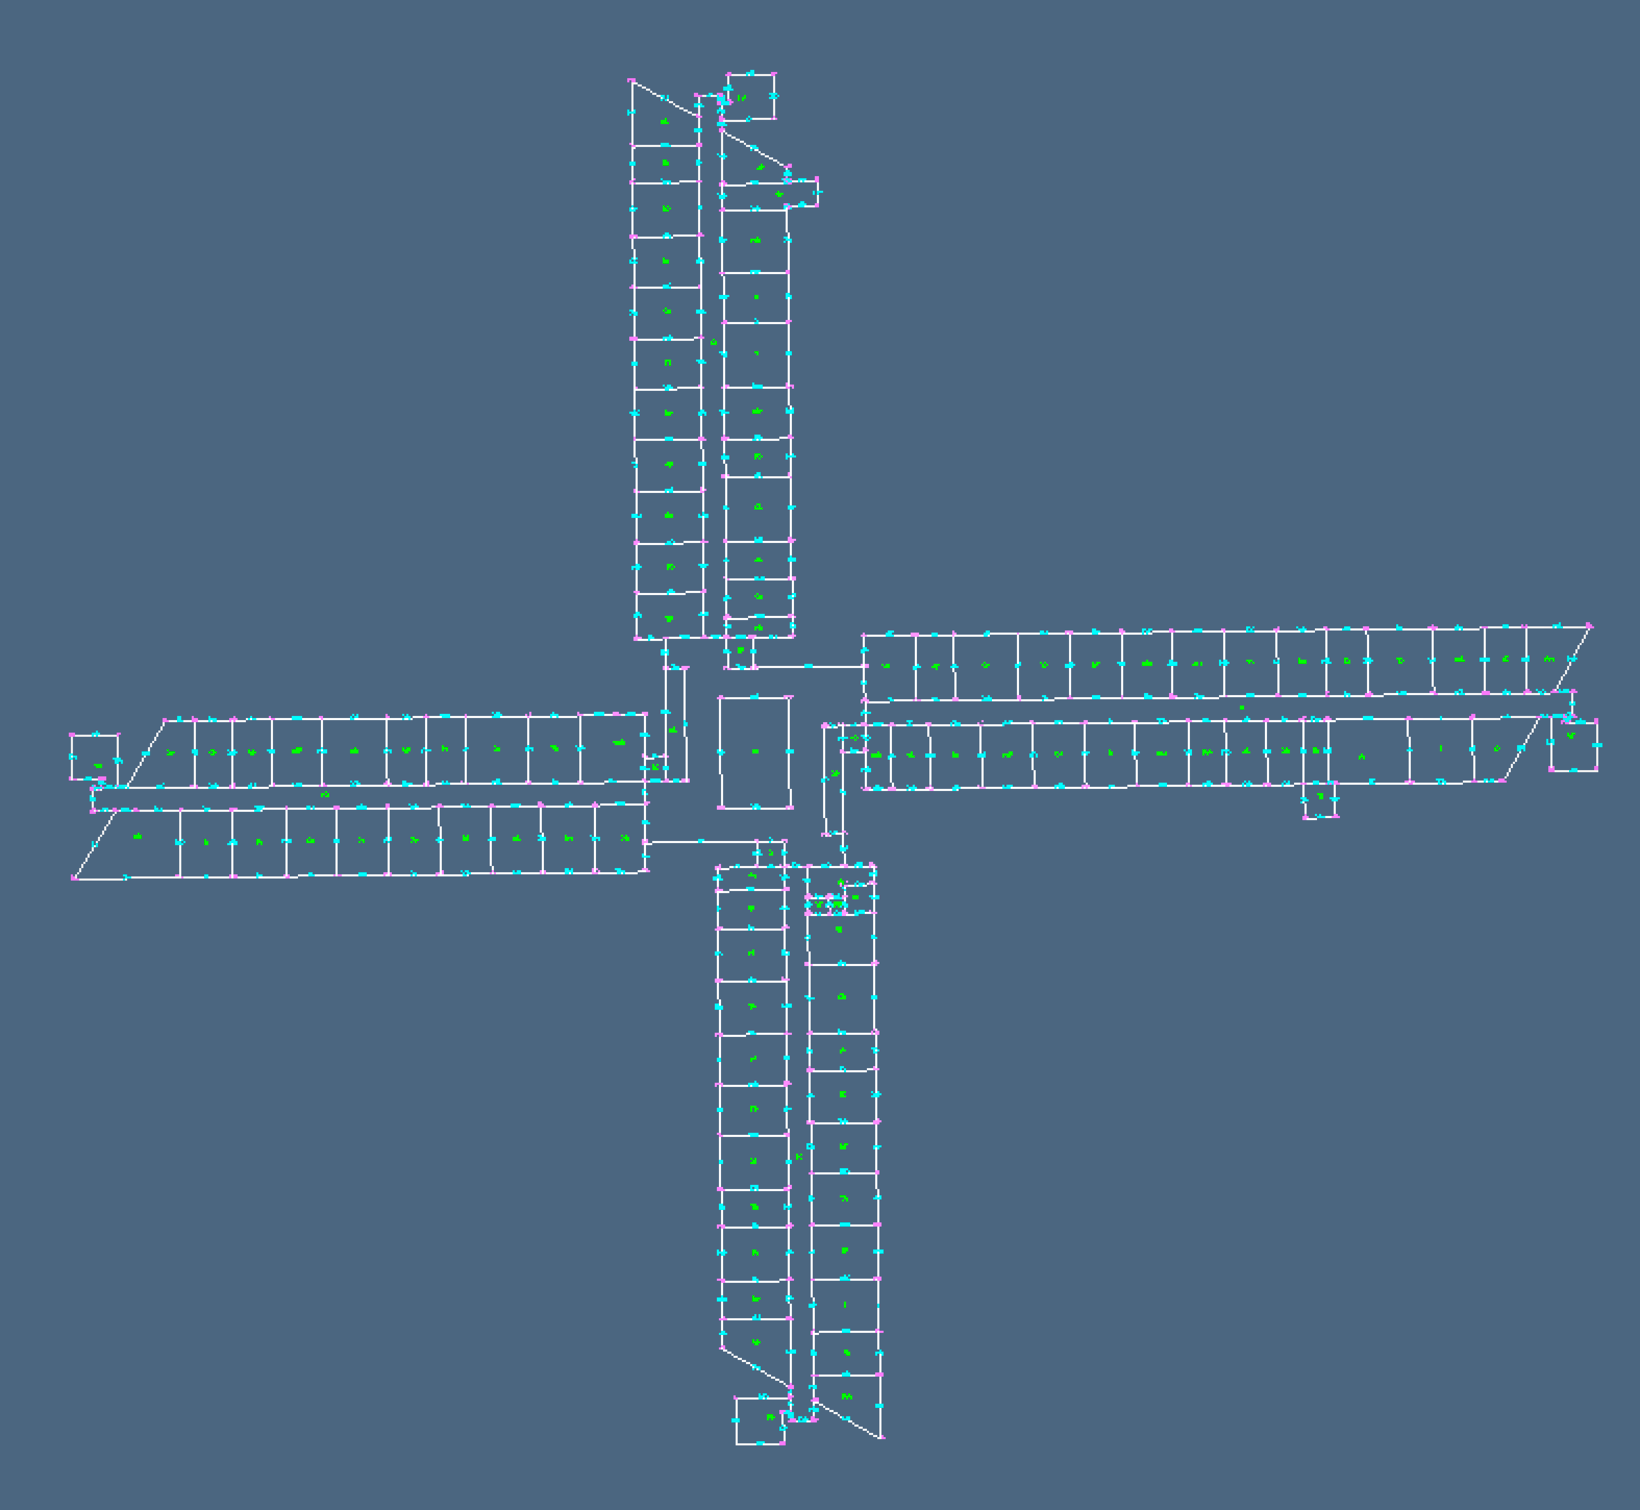
\includegraphics[height=0.325\linewidth,width=0.325\linewidth]{images/torre1} 
   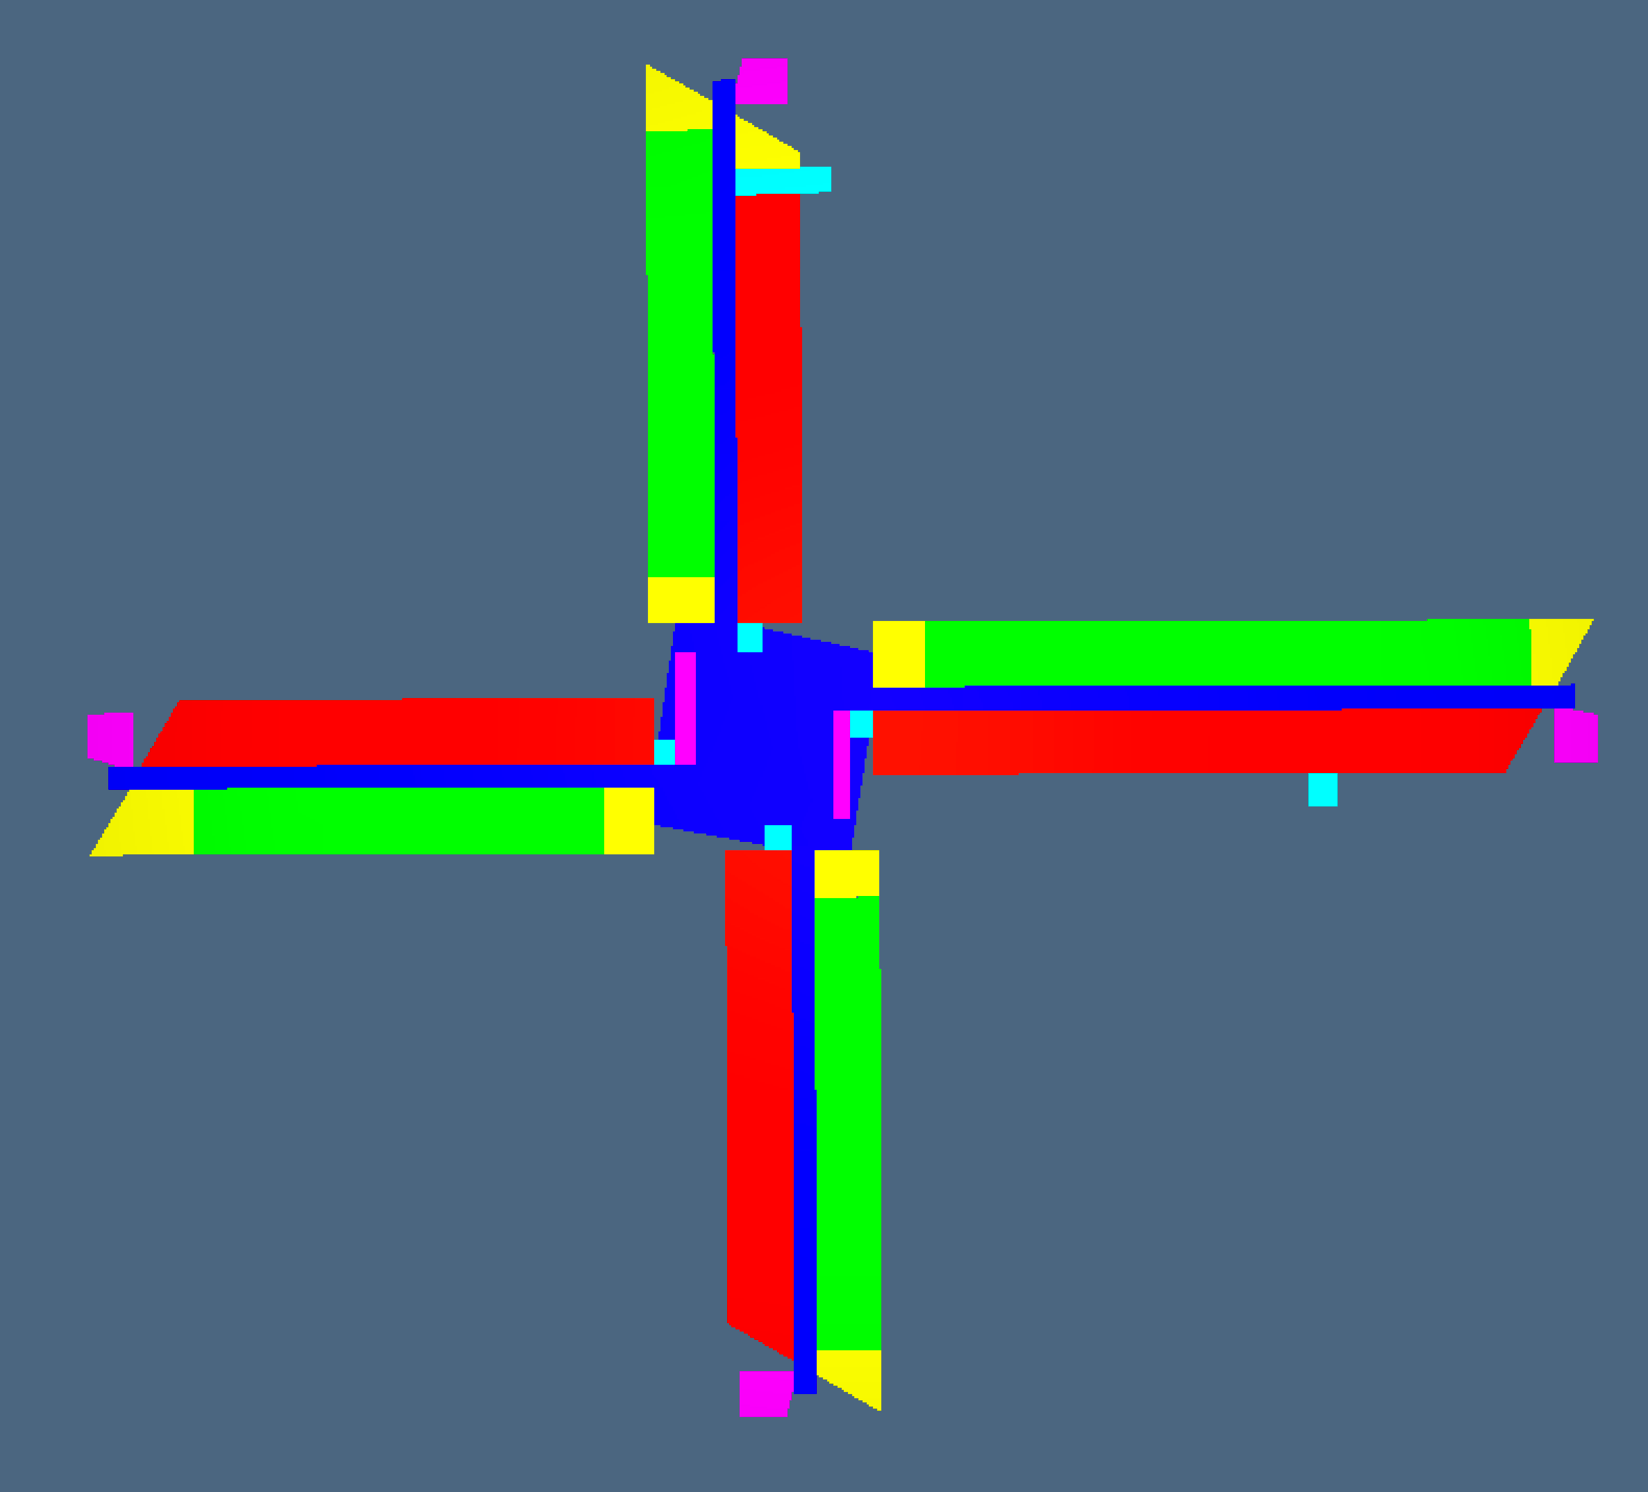
\includegraphics[height=0.325\linewidth,width=0.325\linewidth]{images/torre2} 
   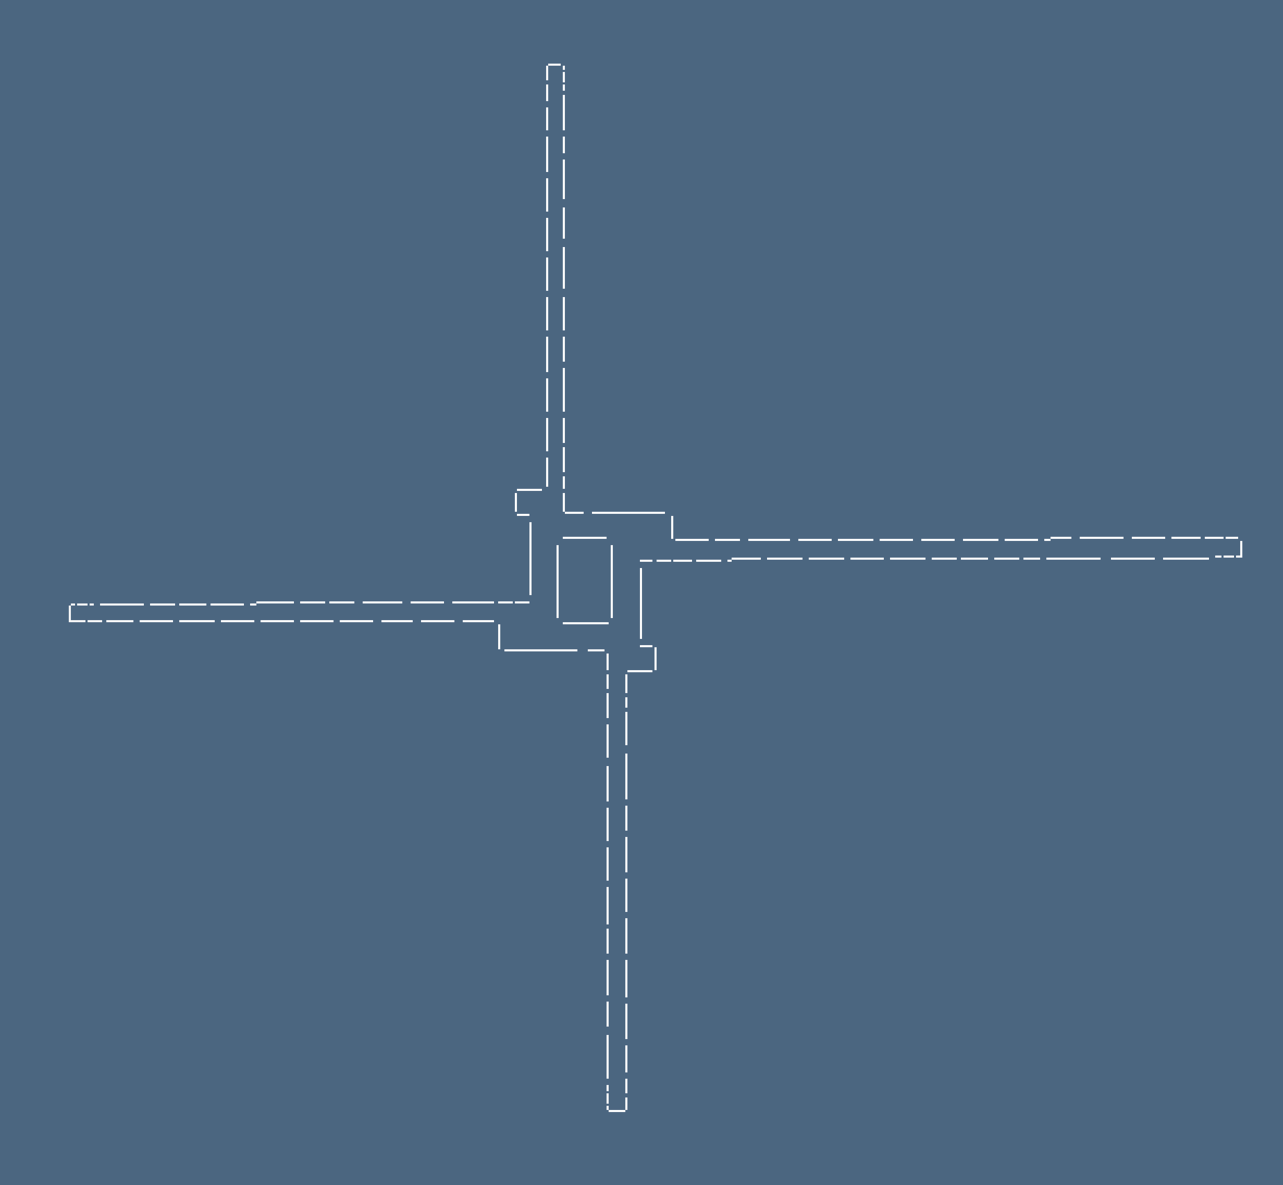
\includegraphics[height=0.325\linewidth,width=0.325\linewidth]{images/torre3} 
   \caption{Edificio torre  per uffici: (a) rappresentazione LAR del piano-tipo come complesso cellulare; (b) ``zooning'' funzionale della planimetria; (c) bordo esploso del 2-complesso definito dalla somma di catene \texttt{piano1-connettivo-orizzontale-zonaNord + piano1-connettivo-orizzontale-zonaSud + piano1-connettivo-orizzontale-zonaEst + piano1-connettivo-orizzontale-zonaOvest + piano1-connettivo-orizzontale- centroStella}.}
   \label{fig:example}
\end{figure}


\end{document}  import sys

